\documentclass{article}
\usepackage{amsmath}
\usepackage{graphicx}

\title{BerichtTitle}
\date{22.06.2020}
\author{Simon Pirkl, Andreas Rohrbach}

\begin{document}

\maketitle

\begin{center}
	
\includegraphics[height=10mm]{./img/ci/HSWT_Logo_gruen.png}

	\vspace{5mm}
	Department of Bioengineering Sciences, Bioprocess Informatics
\end{center}

% \newpage

\tableofcontents
\newpage

\section{Stuff / Ideas / Todos}

\subsection{Topic}
\subsubsection{Research question}
Watson et al derive their results from an evolutionary model containing a single representative individual undergoing individual mutations, motivating this model from the assumption of SSWM (strong selection, weak mutation). Do their results still hold in a more realistic model of evolution involving sexual recombination?

\subsubsection{Adaptive theory}
Watson et al’s central result is that correlations in their single gene regulation network evolve according to Hebb’s rule: if evolution selects a correlation of multiple gene states, those gene states will also become developmentally correlated. Since mutation and sexual recombination generate greater genetic variation, this could lead to correlations evolving not in accordance with Hebb's rule. However, we postulate that Hebb’s rule is driven not by mutation and recombination, but by selection.

\subsubsection{Research hypothesis}
If we reproduce Watson et al’s experiment 1 (single selective environment) for a network population with mutation and recombination, and our adaptive theory is correct, we predict that Hebb’s rule will apply to the evolved networks.

% \subsection{cheat sheet}
% include a graphic:

% \begin{figure}[h!]
% 	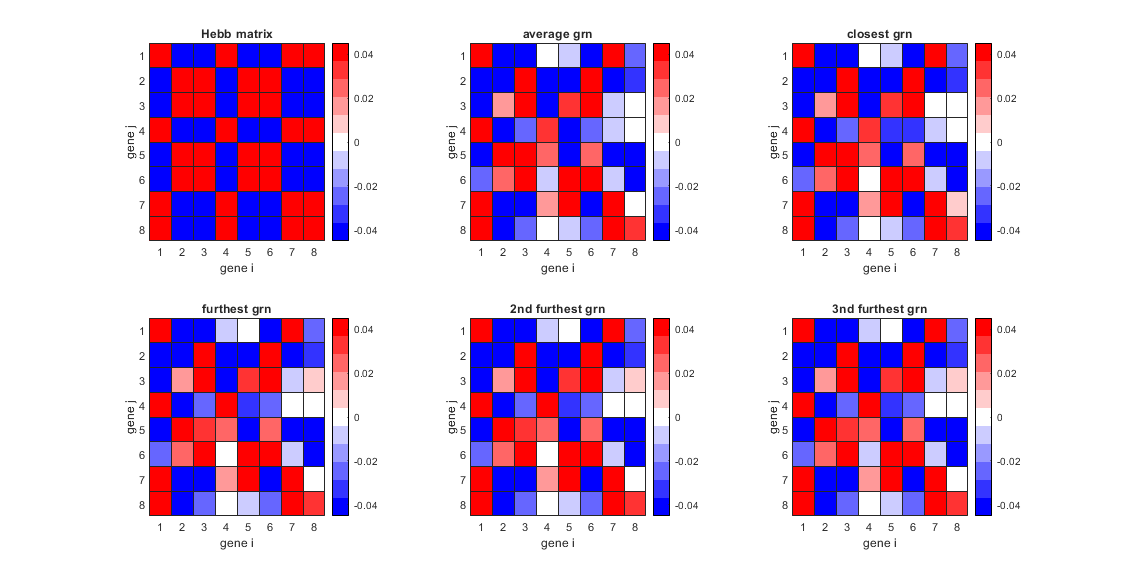
\includegraphics[width=\linewidth]{./img/dummy.jpg}
% 	\caption{This is just a dummy graphic}
% 	\label{fig:dummy}
% \end{figure}


% some inline math: $f(x) = \sqrt{4*\pi}$ , or not:
% \begin{equation}
% 	f(x) = \frac{x^2}{7x}
% \end{equation}

% matrices:
% \begin{equation}
% \left[
% \begin{matrix}
% 1 & 0 & 1\\
% 0 & 1 & 0
% \end{matrix}
% \right]
% \end{equation}

\section{Abstract}

Watson et al. investigated the evolution of phenotypic correlations and "developmental memory". In one of their experiments, an evolutionary model was simulated, containing a single representative individual undergoing individual mutations. This simplification is legit under the assumption of SSWM (strong selection, weak mutation). 
To verify their results in a more realistic model of evolution involving sexual recombination, the experiment was replicated with a more sophisticated fitness evaluation and simple sexual recombination.

- summarize results?

\section{Introduction}

The phenotypic variants we observe are not purely a product of their genes, but of multiple factors, with developmental processes being one of them. In the work of Watson et al., the evolution of a network of recurrent nonlinear ontogenetic interactions was investigated. Such a network could represent a gene regulation network. In their work, multiple experiments were conducted to better understand the evolution of such networks. In the first experiment, the basic effect of selection on interaction coefficients as a function of a single selective environment was assessed. This experiment was conducted under the assumptions of SSWM (strong selection, weak mutation), under which it is sufficient to model the evolution of just one representative individual undergoing individual mutations. 


\section{Foundation}

- (evo devo)
- grns
- grn as matrix
- hebb


\section{Methods}

- traits, genotype and phenotype as column vector with values in [-1; 1]
- formulas for:
	- evolution of phenotype
	- selection and recombination
	- mutation
	- hebb



\section{Results}

- for these parameters, this output
- simulation with differing population sizes (common target)

\section{Discussion}

- interpret results
- so much gentic variation, that genes are more important than grn?
- from where parameters like 1/15 for mutational rate of gene to grn?
- when in later generations more frequencies are quite fit, maybe the selective pressure should increase to reach even better grns
- more experiments from watson14 should be verified with this more realistic model of evolution

\newpage


\begin{appendix}
  \listoffigures
  \listoftables
\end{appendix}

\end{document}
